% 图 5.17 中子散射几何与仪器：(a) 布拉格散射 (b) 矢量三角形 (c) 劳厄扇 (d) 德拜-谢乐锥
% (e) 反应堆谱仪 (f) 散裂源谱仪
\documentclass[tikz,border=5pt]{standalone}
\usetikzlibrary{arrows.meta,calc}
\usepackage{amsmath}
\usepackage{bm}
\usepackage{fontspec}
\setmainfont{Times New Roman}
\begin{document}
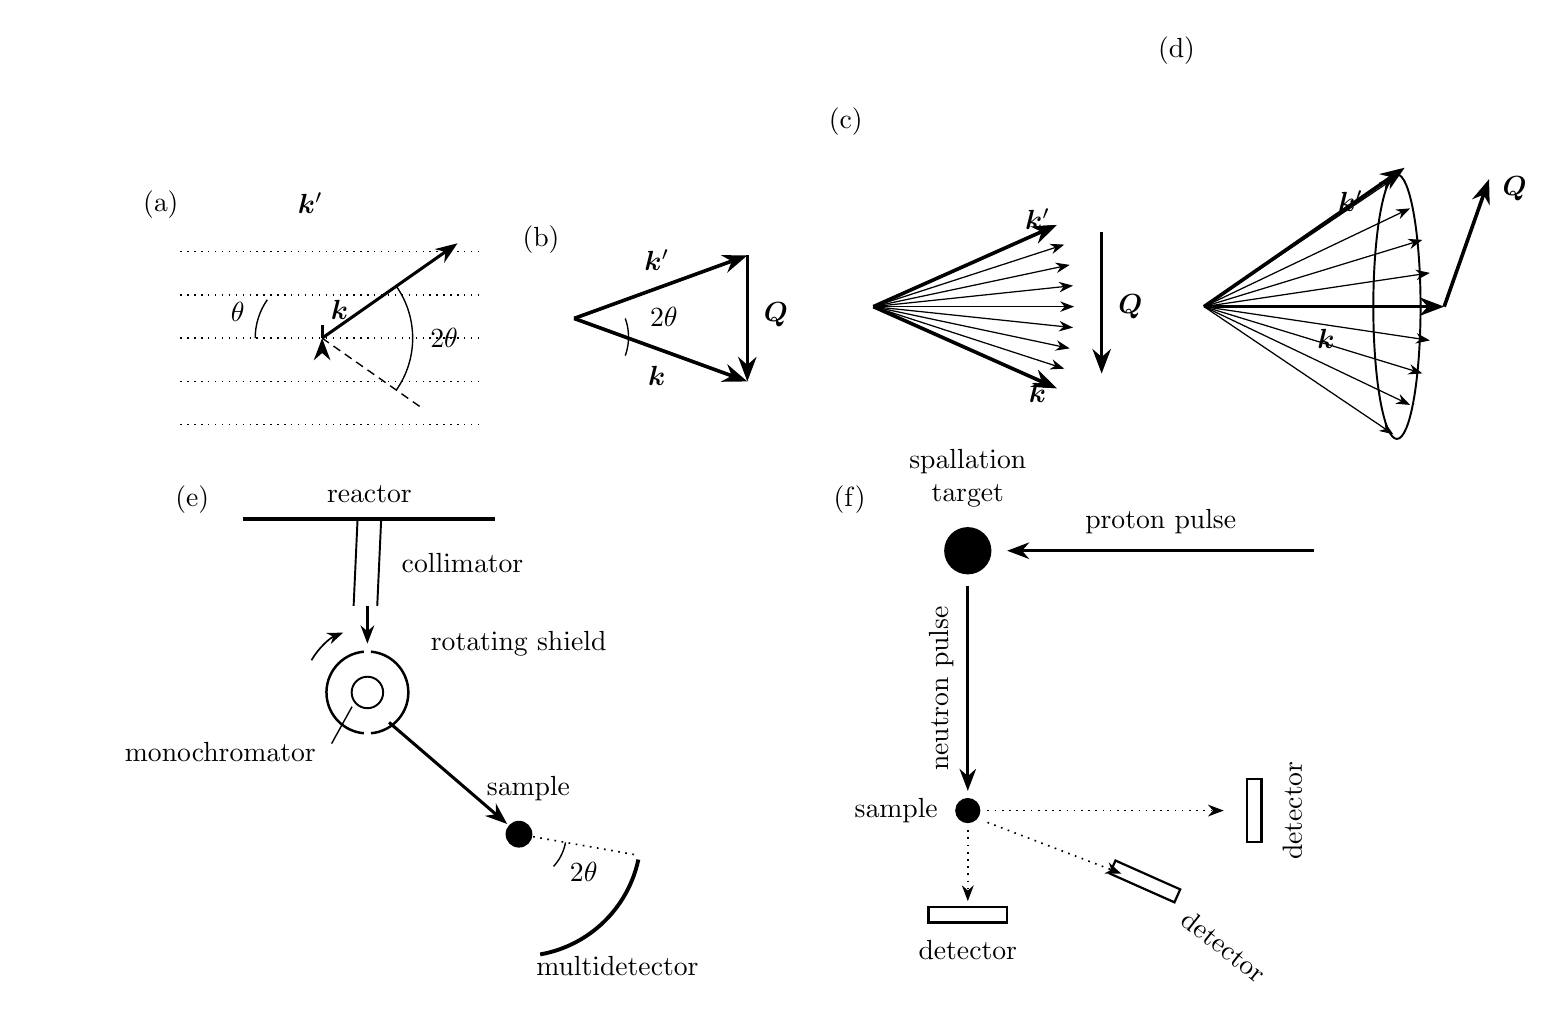
\begin{tikzpicture}[line width=0.8pt,>=Stealth]
% ================= row 1 =================
% ---------- (a) Bragg scattering at lattice planes ----------
\begin{scope}[shift={(0,0)}]
  \foreach \k in {0,0.55,1.1,1.65,2.2}{
    \draw[dotted,line width=0.5] (0.2,\k) -- (4.0,\k);}
  \coordinate (V) at (2.0,1.1);
  \draw[->,line width=1.1] (145:0)+(2.1*cos 145,2.1*sin 145)+(2.0,1.1) coordinate (S)
      -- (V);
  \node[above] at ($(S)!0.5!(V)+(0.22,0.10)$) {$\bm{k}$};
  \draw[->,line width=1.1] (V) -- ++(35:2.1) node[above] at ($(V)+(-0.15,1.45)$) {$\bm{k}'$};
  \draw[dash pattern=on 3pt off 2pt,line width=0.5] (V) -- ++(-35:1.55);
  \draw[line width=0.5] ($(V)+(180:0.85)$) arc[start angle=180,end angle=145,radius=0.85];
  \node at ($(V)+(163:1.12)$) {$\theta$};
  \draw[line width=0.5] ($(V)+(-35:1.15)$) arc[start angle=-35,end angle=35,radius=1.15];
  \node at ($(V)+(0:1.55)$) {$2\theta$};
  \node at (-0.05,2.8) {(a)};
\end{scope}
% ---------- (b) vector triangle ----------
\begin{scope}[shift={(5.2,1.35)}]
  \draw[->,line width=1.3] (0,0) -- (2.2,-0.8);
  \draw[->,line width=1.3] (0,0) -- (2.2,0.8);
  \draw[line width=0.5] (0.65,0) arc[start angle=20,end angle=-20,radius=0.69];
  \node at (1.14,0.02) {$2\theta$};
  \draw[->,line width=1.3] (2.2,0.8) -- (2.2,-0.8);
  \node[above] at (1.05,0.48) {$\bm{k}'$};
  \node[below] at (1.05,-0.48) {$\bm{k}$};
  \node[right] at (2.28,0.05) {$\bm{Q}$};
  \node at (-0.42,1.0) {(b)};
\end{scope}
% ---------- (c) Laue fan ----------
\begin{scope}[shift={(9.0,1.5)}]
  \foreach \a in {-24,-18,-12,-6,0,6,12,18,24}{
    \draw[->,line width=0.45] (0,0) -- (\a:2.55);}
  \draw[->,line width=1.3] (0,0) -- (-24:2.55);
  \draw[->,line width=1.3] (0,0) -- (24:2.55);
  \node[above] at (22:2.25) {$\bm{k}'$};
  \node[below] at (-22:2.25) {$\bm{k}$};
  \draw[->,line width=1.3] (2.9,0.95) -- (2.9,-0.85);
  \node[right] at (2.98,0.0) {$\bm{Q}$};
  \node at (-0.35,2.35) {(c)};
\end{scope}
% ---------- (d) Debye-Scherrer cone ----------
\begin{scope}[shift={(13.2,1.5)}]
  \foreach \a in {-34,-25.5,-17,-8.5,8.5,17,25.5,34}{
    \draw[->,line width=0.45] (0,0) -- (\a:2.9);}
  \draw[->,line width=1.3] (0,0) -- (0:3.05);
  \draw[->,line width=1.3] (0,0) -- (34.7:3.1);
  \draw[line width=0.7] (2.45,0) ellipse [x radius=0.30, y radius=1.68];
  \node[below] at (1.55,-0.16) {$\bm{k}$};
  \node[above] at (30:2.15) {$\bm{k}'$};
  \draw[->,line width=1.3] (3.05,0) -- (3.62,1.62);
  \node[right] at (3.66,1.5) {$\bm{Q}$};
  \node at (-0.35,3.25) {(d)};
\end{scope}
% ================= row 2 =================
% ---------- (e) reactor source instrument ----------
\begin{scope}[shift={(0,-6.2)}]
  \draw[line width=1.3] (1.0,5.0) -- (4.2,5.0);
  \node[above] at (2.6,5.08) {reactor};
  \draw[line width=0.7] (2.45,5.0) -- (2.4,3.9);
  \draw[line width=0.7] (2.75,5.0) -- (2.7,3.9);
  \node[right] at (2.88,4.45) {collimator};
  \draw[->,line width=0.8] (2.575,3.9) -- (2.575,3.42);
  \draw[line width=0.7] (2.575,2.8) circle (0.20);
  \draw[line width=0.9] ($(2.575,2.8)+(95:0.52)$) arc[start angle=95,end angle=265,radius=0.52];
  \draw[line width=0.9] ($(2.575,2.8)+(-85:0.52)$) arc[start angle=-85,end angle=85,radius=0.52];
  \draw[->,line width=0.6] ($(2.575,2.8)+(150:0.82)$) arc[start angle=150,end angle=112,radius=0.82];
  \node[right] at (3.25,3.42) {rotating shield};
  \node[anchor=east] at (2.05,2.05) {monochromator};
  \draw[line width=0.5] (2.12,2.15) -- (2.38,2.62);
  \draw[->,line width=1.1] (2.85,2.42) -- (4.35,1.13);
  \fill (4.5,1.0) circle (0.17);
  \node[above=2pt] at (4.62,1.22) {sample};
  \draw[dotted,line width=0.6] (4.5,1.0) -- ++(-10:1.55);
  \draw[line width=0.5] ($(4.5,1.0)+(-43:0.6)$) arc[start angle=-43,end angle=-10,radius=0.6];
  \node at ($(4.5,1.0)+(-30:0.95)$) {$2\theta$};
  \draw[line width=1.4] ($(4.5,1.0)+(-80:1.55)$) arc[start angle=-80,end angle=-12,radius=1.55];
  \node[below] at (5.75,-0.42) {multidetector};
  \node at (0.35,5.25) {(e)};
\end{scope}
% ---------- (f) spallation source instrument ----------
\begin{scope}[shift={(8.6,-6.2)}]
  \fill (1.6,4.6) circle (0.30);
  \node[above,align=center] at (1.6,5.02) {spallation\\target};
  \draw[->,line width=1.1] (6.0,4.6) -- (2.1,4.6);
  \node[above] at (4.05,4.68) {proton pulse};
  \draw[->,line width=1.1] (1.6,4.15) -- (1.6,1.55);
  \node[rotate=90,above=2pt] at (1.62,2.85) {neutron pulse};
  \fill (1.6,1.3) circle (0.16);
  \node[left] at (1.35,1.3) {sample};
  % detectors
  \draw[dotted,line width=0.6,->] (1.85,1.3) -- (4.85,1.3);
  \draw[line width=0.8] (5.15,0.9) -- (5.15,1.7) -- (5.33,1.7) -- (5.33,0.9) -- cycle;
  \node[rotate=90] at (5.72,1.3) {detector};
  \draw[dotted,line width=0.6,->] (1.85,1.15) -- (3.55,0.50);
  \begin{scope}[shift={(3.85,0.40)},rotate=-24]
    \draw[line width=0.8] (-0.45,-0.09) rectangle (0.45,0.09);
  \end{scope}
  \node[rotate=-38] at (4.85,-0.42) {detector};
  \draw[dotted,line width=0.6,->] (1.6,1.05) -- (1.6,0.15);
  \draw[line width=0.8] (1.1,-0.12) rectangle (2.1,0.08);
  \node[below] at (1.6,-0.22) {detector};
  \node at (0.1,5.25) {(f)};
\end{scope}
\end{tikzpicture}
\end{document}
